
\section{Molecular biology of the bladder}


To understand cancer, we need to know how the cells work and replicate in the tissues, which is only possible by studying the constituent blocks that are represented or regulated by proteins, which in turn are created by the instructions from DNA. To find the faulty biological processes the analysis needs to be performed on both the tumorous and healthy cells/tissue enabling the comparison between normal and abnormal behaviour. To do this, scientists use multiple streams of information from molecular biology which includes gene expression (transcriptomics), mutations (genomics), lipidomics, proteomics and others. Through this existing biological data combined with modelling, researchers are creating linkings such as gene network interactions. 

% introduction to DNA & RNA, the genetic diversity on Earth, why it's important and some fascinating facts
A useful analogy for engineers is that a DNA molecule is the equivalent of a hard drive where information is stored, while the RNA is similar to RAM. This represents the relevant information (from the DNA) needed to make new copies of a particular protein. Even though all the living organisms share a large amount of DNA, each species has its features\footnote{Interestingly the same mechanism to build proteins is present in animals, plants and is highly similar in bacteria and other living organisms.}. Across a species, the genetic material varies slightly making the individual both unique and common, depending on the reference point. Interestingly, at birth the cells of an individual share the same genetic information, but as it ages the new cells created will start to have anomalies specific to tissue. Cancerous tissue has an uncommonly large number of these changes.

\begin{figure}[!ht]
  \centering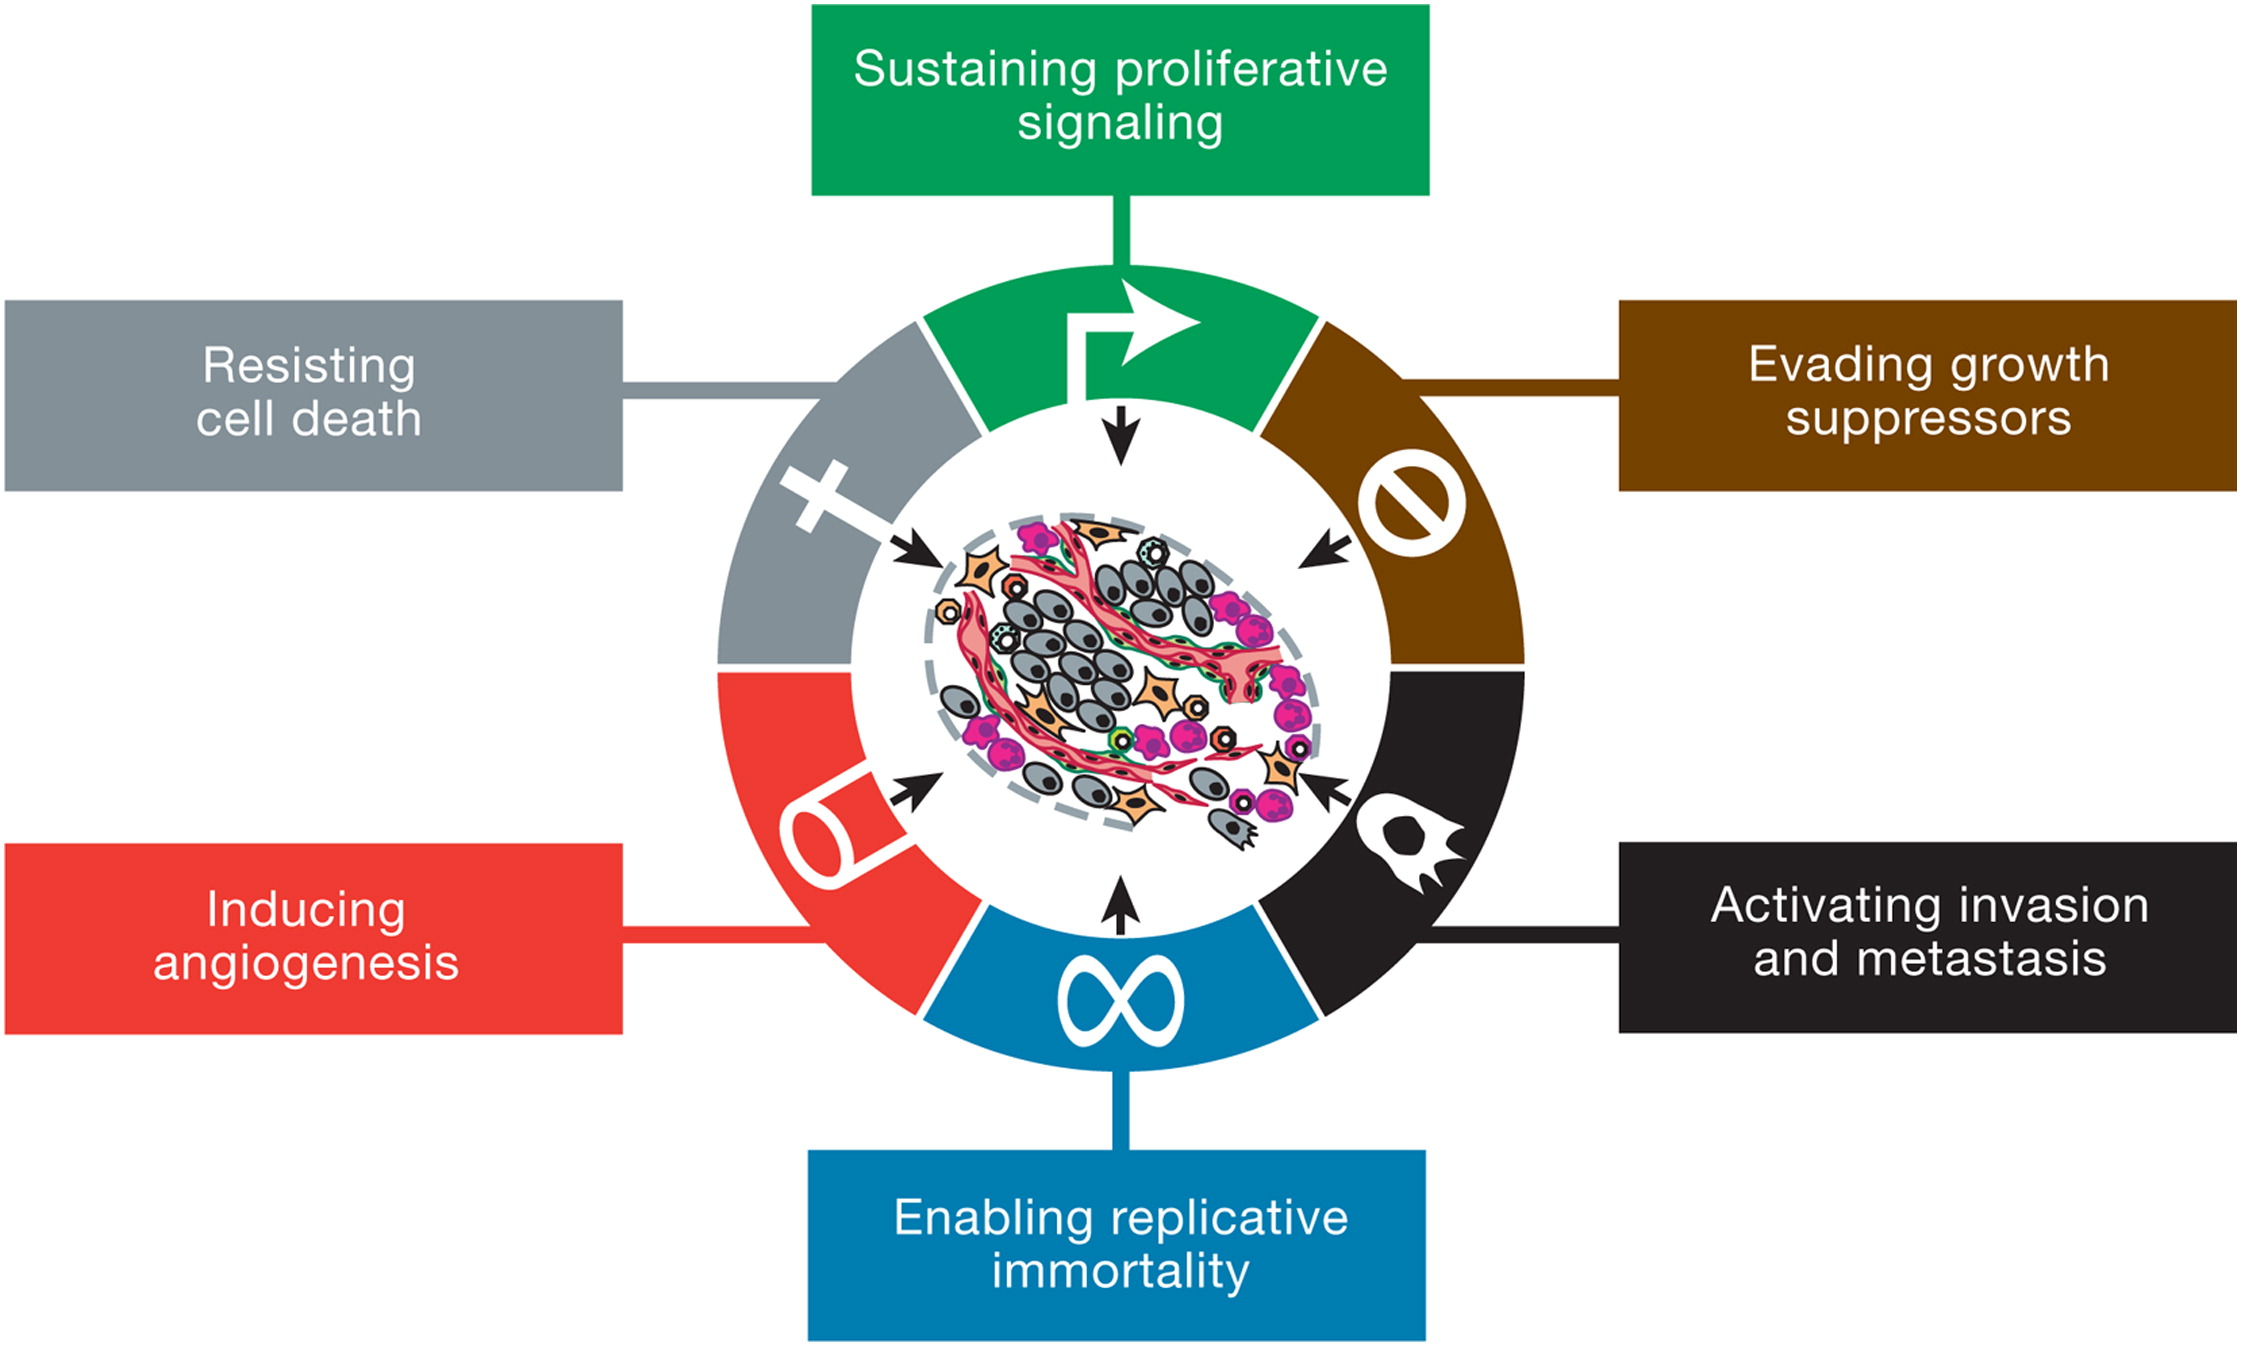
\includegraphics[width=0.8\textwidth,height=0.8\textheight,keepaspectratio]{Images/TCGA/tumour_causes}
    \caption{Hallmarks for the cancer tumours\cite{Hanahan2011-px}. The Sustaining proliferative signalling feature means that the cancerous cell will be 'encouraged' to divide while evading the growth suppressors and resist cell death will only aid the birth of new malign cells. On top of that, these cells have the replicative immortality trait. Activating invasion and metastasis means that the cells are capable of spreading to other parts of the body. Lastly, angiogenesis refers to the tumours capability to draw nutrients to sustain itself through the creation of blood vessels. }
    \label{fig:hallmarks_cancer}
\end{figure}

% Small paragraph showing the ideas
Numerous sources are causing genetic alterations in a healthy organism which can lead to diseases. From \cref{fig:hallmarks_cancer} it can be seen that a large proportion of the tumour hallmarks are related to the cell division cycle that is because of all the properties of a cell, this is the one that comes under most natural selection because it leads to growth/expansion of the tumour. From evading growth suppressors to resisting cell death, the cancerous cell will not stop dividing and will slowly conquer the tissue as the healthy cells will reach the end of their cycle and die.

A driving motivation in cancer research is to learn the gene mechanisms to develop a cure for the disease. Medicine made important progress in cancer research \& diagnosis but cancer remains an unsolved problem. One of the reasons for this is the intricate mechanism of gene interactions that due to its complexity is difficult to understand. On top of that, it is not feasible to collect the ideal data\footnote{The ideal genomic dataset is represented by a large number of tumour samples, matched with a blood sample, and multi-omic sequenced (proteins, RNA, mutations etc.). Multiple samples from the same donor to track genetic changes as the disease progress and map it to the appropriated genes.)} to make accurate predictions; imagine a person suffering from cancer and scientists constantly asking for more data (i.e. biopsy). Thus, due to both ethical and clinical considerations, samples are typically taken at the point of cancer surgery, so repeat samples are usually impracticable . Therefore, it is challenging to determine the exact gene interactions which drive a subtype of cancer and as a matter of fact, any disease. 
% introducing the datasets and the efforts to get data that may be useful for us. This includes:
%  expression, mutation and signalling 
Sequencing techniques are becoming more affordable every year, and now companies like 10X Genomics can extract gene expression information at the single cell level. In addition, we get mutation data with base-pair precision; i.e. we know which part of the gene sequence presents an anomaly. Even with the costs lowering every year, sequencing large cohorts is expensive, and there are just a few large studies such as The Cancer Genome Atlas which has been used in this project.

There are two important types of datasets used in this project: the data on non-cancerous bladder from Jack Birch Unit (JBU) and MIBC cohort from The Cancer Genome Atlas (TCGA). The first helps build a representation of the urothelium which is as close as possible to the healthy tissue\footnote{As it is an invasive procedure, it is extremely challenging to convince a healthy person to donate a bladder tissue biopsy} which is then use to inform the tumour stratification.

\cref{s:lit:bladder_cancer} introduces the reader to the bladder cancer by providing an overview of the global and local impact of the disease to both the patients and the healthcare system. It also presents the molecular characteristics of the bladder cancer and what is known at the moment of writing. The chapter then continues with an introduction of the non-cancerous dataset with the molecular properties.

\subsection{Bladder Cancer} \label{s:lit:bladder_cancer}
% Overview of the bladder cancer stats
According to Cancer Research UK, bladder cancer is the 10th most common cause of cancer and the 11th most common cancer in the UK \cite{Cancer_Research_UK2015-cf}. This is equivalent to $\sim10,000$ cases from which  $\sim5000$ are deaths, with a 5-year survival rate of 52.6\%. In 2008\cite{Ferlay2010-sx} the worldwide estimates for bladder cancer was $\sim380,000$ new cases and $\sim150,000 $deaths per year. In 2020\cite{Sung2021-hn} , there were $\sim573,000$ cases with $\sim212,536$ deaths reported which shows a considerable increase in the cancer cases\footnote{A good resource to get an overview of the prevelance of bladder cancer (and other cancers too) is the website from World Health Organisation, particularly the trends in cancer overtime: \href{https://gco.iarc.fr/en}.}. Men are 3 times more likely to develop bladder cancer and bladder cancer is specific to Western countries \cite{Knowles2015-mu}. 

% Talk about bladder cancer causes, economical burden
One of the main causes of bladder cancer is caused by smoking, being thought to provoke 50\% of the cases \citet{Knowles2015-mu}. However, the underling biological process on how smoking causes cancer is not understood. Other environment risk factors are metal contamination such as arsenic-water or exposure to ionising radiation \citet{Knowles2015-mu}. 

% Types ands stages of bladder cancer
There are multiple systems to classify bladder depending on their utility. For medical doctors there are two popular systems to dichotomies the bladder cancer Tumour-Node-Metastasis (TNM) and the Internail Sociecty of Urological Pathology (ISUP). The stages of the bladder cancer and the two naming conventions can be seen in \cref{fig:lit:bladder_cancer_stages}; image taken from the bladder cancer review from \citet{Knowles2015-mu}. The figure should be taken as an illustration of the stages and their classification, and not as the evolution of the bladder cancer.

\begin{figure}[!htb]    
    \centering
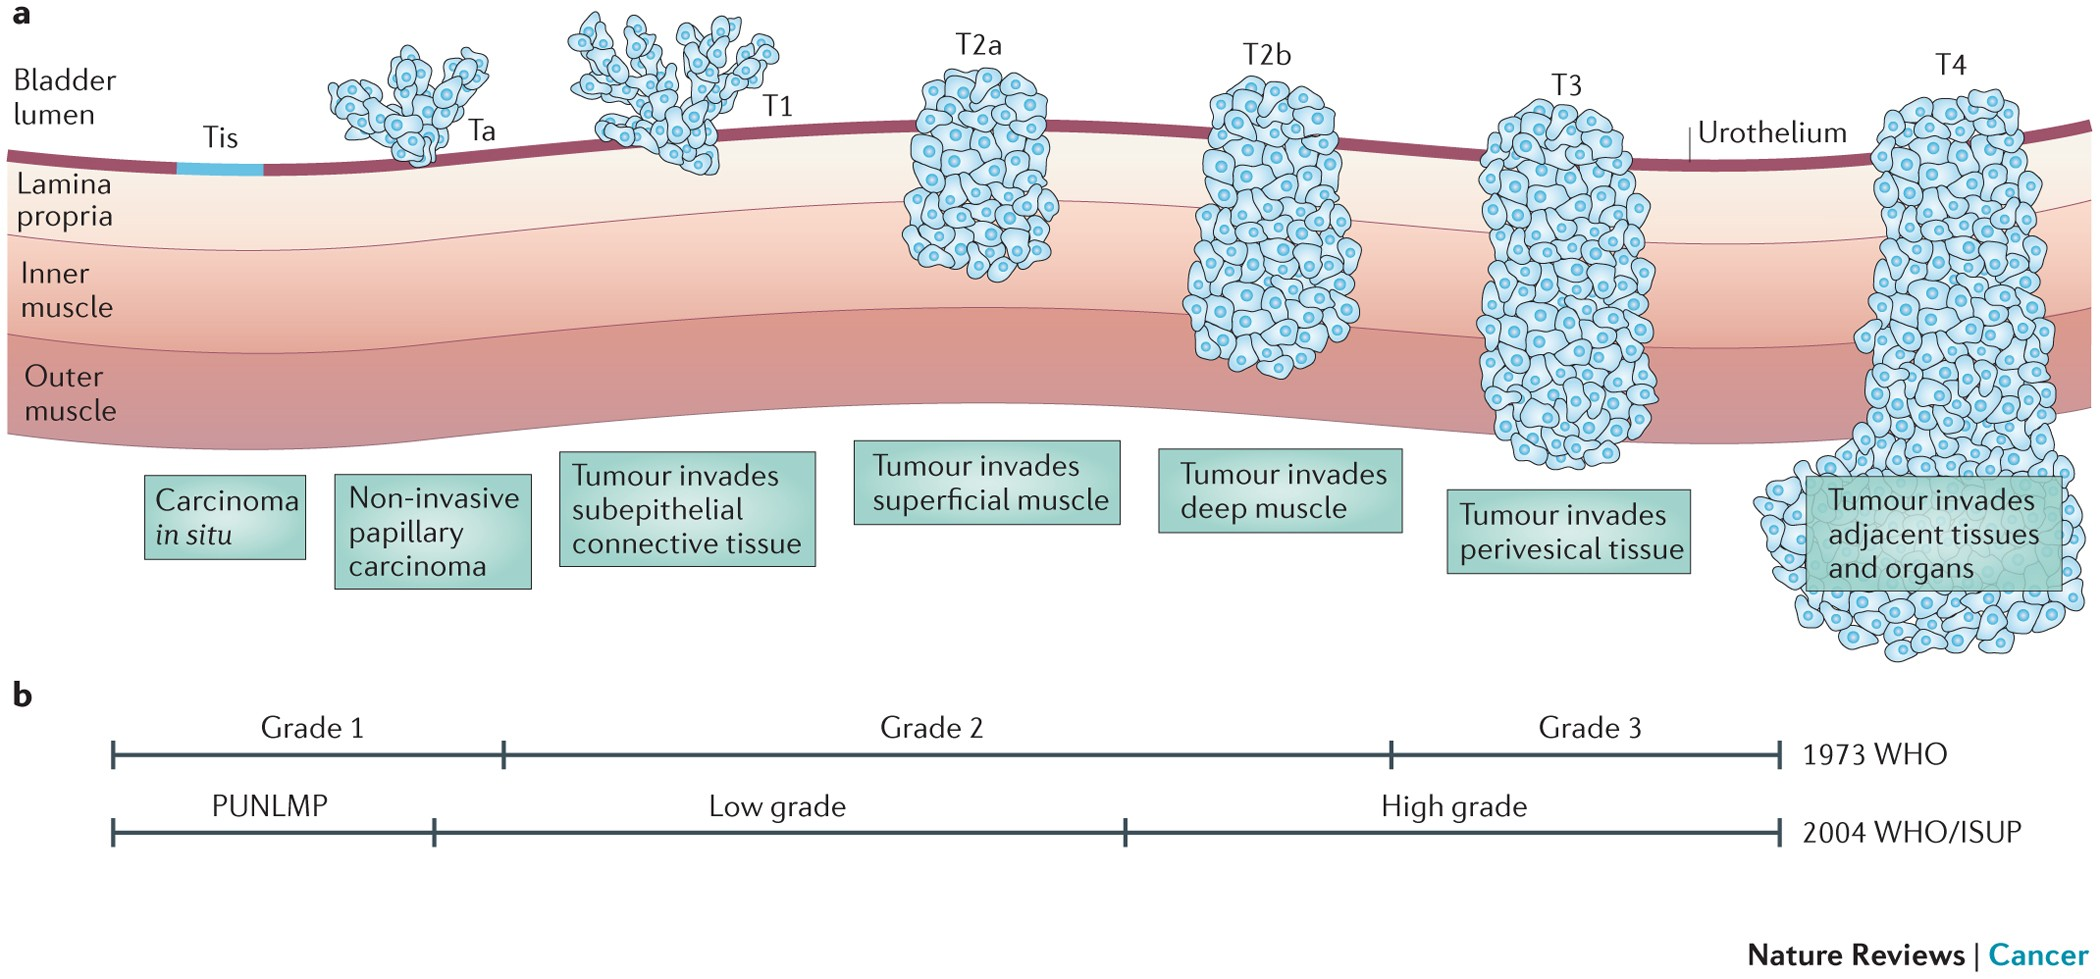
\includegraphics[width=0.9\textwidth,height=0.9\textheight,keepaspectratio]{Sections/Lit_review/Resources/bladder_cancer_grading.jpg}
    \caption{"Bladder cancer grading and staging" from \cite{Knowles2015-mu}. It displays the two grading of the bladder cancer based on its stage. Image a) should be taken just as an illustration of the different stages of bladder cancer and not mistaken with the disease evolution. }
    \label{fig:lit:bladder_cancer_stages}
\end{figure}


There are two main types of bladder cancer: non-muscle invasive (NMIBC) and muscle-invasive bladder cancer (MIBC). From \cref{fig:lit:bladder_cancer_stages} stages Tis, Ta and T1 are classified as NMIBC as they do not invaded the muscle. NMIBC appears in $\sim70\%$ of the bladder patients, it has a high 5-year survival rate with $\sim90\%$, it frequently recurs in 50-70\% of the cases and only 10-15\% progress to muscle invasion \cite{Knowles2015-mu}. Thus, patients suffering from this type of bladder cancer have favourable prognostics but their quality of life is impact as they need to attend periodical cystocopies checkups.

The muscle invasive bladder cancer encompass the T2a, T2b, T3 and T4 stages and it appears in $\sim30\%$ of the bladder cancer cases. It is more aggressive than the NMIBC with $\sim50\%$ 5-year survival prognosis, almost half of the cases of MIBC develop metastasis and for these patients the median survival is 12-15 months\cite{Knowles2015-mu}. Usually the metastatic sites for bladder cancer are lung, livers and the bones.

The patients diagnosed with MIBC undergo cystectomy which removes the entire bladder and has a larger impact to quality of life, while the NIMBC patients have regular cystocopies checkups. Both procedures have a negative impact of the patients and carer's quality of life, and bring an financial burden to them and the healthcare system. Thus, there is a need to develop better diagnosis tools and treatment plants for bladder cancer, especially for the MIBC.

\paragraph*{MIBC subtyping}

% Introduction of TCGA
There are two comprehensive studies of the muscle-invasive bladder cancer (MIBC) cohort from The Cancer Genome Atlas (TCGA) \citet{Tcga2014-dr} and \citet{Robertson2017-mg}. The first is the initial research analysing the fist batch of patient samples (131) while the other analysed the entire cohort of 412 patient samples. The MIBC cohort from TCGA is an invaluable asset for the research community as a number of sequencing techniques were applied to the samples: mRNAseq (gene expression), WEX and WGS (somatic mutations), microarray-based (copy number variations) as well as metadata about the patients. This cohort is characterised by aggressive tumours, having a high grade muscle invasive.

% Talk about the TCGA subtypes
In the work of \citet{Robertson2017-mg} multiple data types are analysed separately, centring on the subgroups derived from gene expression and then correlating with the other data analysis. The main result being the stratification of the MIBC into five distinct molecular subtypes: $35\%$- Luminal Papillary (LumP), $19\%$ Luminal infiltrated (LumInf), $6\%$ Luminal, $35\%$ Basal Squamous (Ba/Sq) and $5\%$ Neuronal. The highest 5-year survival is given by the Luminal subgroups while the Neuronal has the worst prognosis. 

% Introduce Lund cohort
Another study of the bladder cancer, but using microarray sequencing to derive gene expression is the work from \citet{Marzouka2018-ge}/

% Introducing the consensus work
TCGA cohort is also part of the consensus effort to stratify the bladder cancer \citet{Kamoun2020-tj}. The consensus combines 6 different dataset of ... 

% Introducing the delays in translating the subtypes to clinical application
Importantly \citet{Kamoun2020-tj} admitted that there are delays in translating the different subtypes discovered through the consensus, TCGA to clinical applications. 


\begin{table}[htbp]
\centering
\caption{The molecular characterisation of the TCGA subgroups from \cite{Robertson2017-mg}}
\begin{tabularx}{\textwidth}{
  >{\hsize=.6\hsize\raggedright\arraybackslash}X
  >{\hsize=.8\hsize\raggedright\arraybackslash}X
  >{\hsize=.6\hsize\arraybackslash}X
}
\toprule
Subtype & Genes & Description \\
\midrule
Luminal-papillary (35\%) & KRT20, PPARG, FOXA1, GATA3, SNX31, UPK1A, UPK2, FGFR3 & 
\begin{itemize}[leftmargin=*, nosep, after=\vspace{-\baselineskip}, before=\vspace{-.6\baselineskip}]
    \item Characterised by FGFR3 mutations
    \item Papillary histology
    \item Low risk of progression
\end{itemize} \\
\midrule
Luminal-infiltrated (19\%) & CD274, PDCD1LG2, IDO1, CXCL11, L1CAM, SAA1 & 
\begin{itemize}[leftmargin=*, nosep, after=\vspace{-\baselineskip}, before=\vspace{-.6\baselineskip}]
    \item Lowest purity
    \item High expression of EMT and myofibroblast markers, and of the miR-200s (tumour suppressor)
    \item Medium expression of CD274 and CTLA4 immune markers
    \item May respond to immune checkpoint therapy
    \item May be resistant to cisplatin-based chemotherapy
\end{itemize} \\
\midrule
Luminal (6\%) & KRT20, PPARG, FOXA1, GATA3, SNX31, UPK1A, UPK2, FGFR3 & 
\begin{itemize}[leftmargin=*, nosep, after=\vspace{-\baselineskip}, before=\vspace{-.6\baselineskip}]
    \item New subtype in TCGA
\end{itemize} \\
\midrule
Basal-squamous (35\%) & CD44, KRT6A, KRT5, KRT14, COL17A1; Squamous: DSC3, GSDMC, TCGM1, PI3, TP63 & 
\begin{itemize}[leftmargin=*, nosep, after=\vspace{-\baselineskip}, before=\vspace{-.6\baselineskip}]
    \item High incidence in women
    \item Squamous differentiation
    \item Basal keratin expression
    \item High expression of CD274 and CTLA4 immune markers
    \item Might be useful for immune checkpoint therapy
\end{itemize} \\
\midrule
Neuronal (5\%) & MSI1, PLEKHG4B, GNG4, PEG10, RND2, APLP1, SOX2, TUBB2B & 
\begin{itemize}[leftmargin=*, nosep, after=\vspace{-\baselineskip}, before=\vspace{-.6\baselineskip}]
    \item Expression of neuroendocrine, neuronal gene and high cell-cycle signature of proliferative state
    \item The most aggressive tumours with the lowest survival rate
\end{itemize} \\
\bottomrule
\end{tabularx}
\end{table}

\subsubsection{Other omics}

% Some properties of the bladder cancer
% - highly mutated, a lot of epginetic changes
The research conducted by \citet{Alexandrov2013-gi} studies the mutational signatures across the human tumour types, covering $\sim7000 $cancer samples from which 20 distinct mutational signatures were extracted. \Cref{fig:lit:cancer_mut_sig} shows the mutation burden across the tumour types, with the skin cancer being the most mutated type. The bladder cancer has the 4th highest mutation burden with Signatures 13, 2 and 5 from COSMIC database\cite{Tate2019-yj}. Signature 2 and 13 are related to APOBEC family activity which are triggered by immune response. Signature 5 is unknown but it is thought to related to the mutations accumulated through ageing. 

\begin{figure}[!htb]    
    \centering
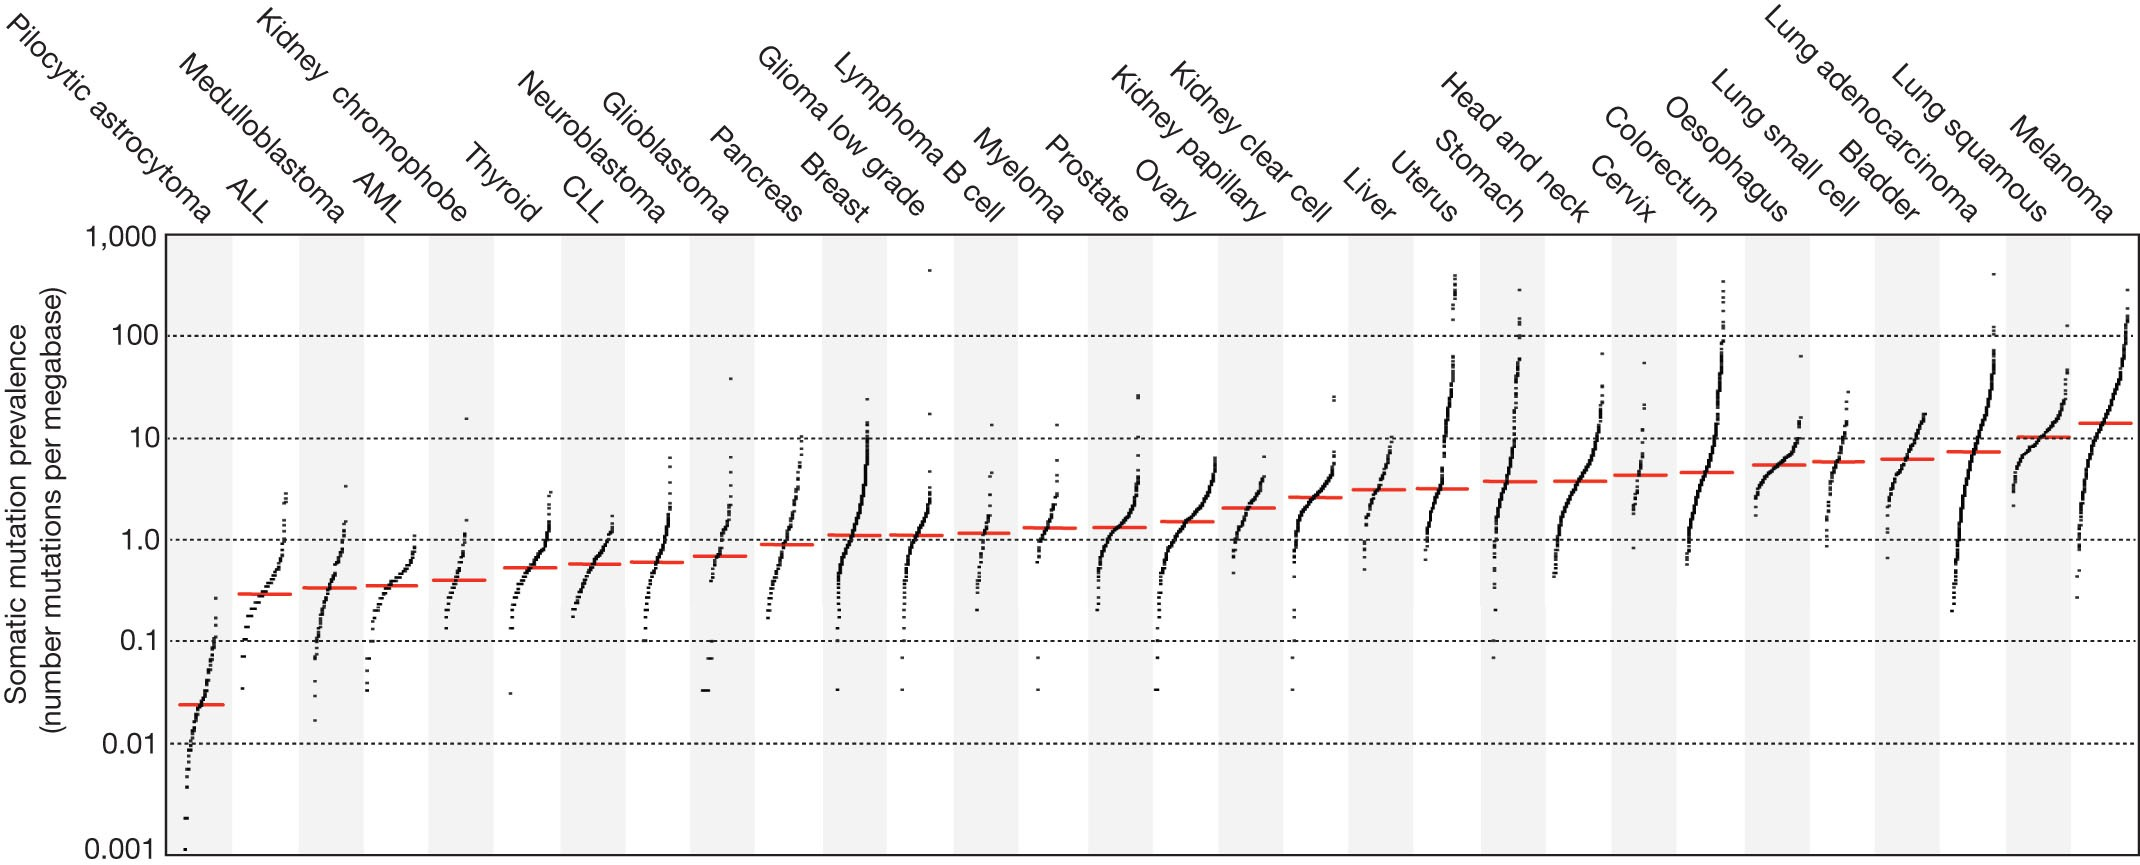
\includegraphics[width=0.9\textwidth,height=0.9\textheight,keepaspectratio]{Sections/Lit_review/Resources/mut_sig_cancers.jpg}
    \caption{Image from \cite{Alexandrov2013-gi} showing the somatic mutations across the different human cancer. Each sample is represented by a dot and the red line is the median number of mutation in that tumour type. The y-axis is the number of mutations per megabases, and the cancer types are ordered by the median mutation count, which makes bladder cancer the 4th highest mutated cancer.}
    \label{fig:lit:cancer_mut_sig}
\end{figure}

\begin{figure}[!htb]    
    \centering
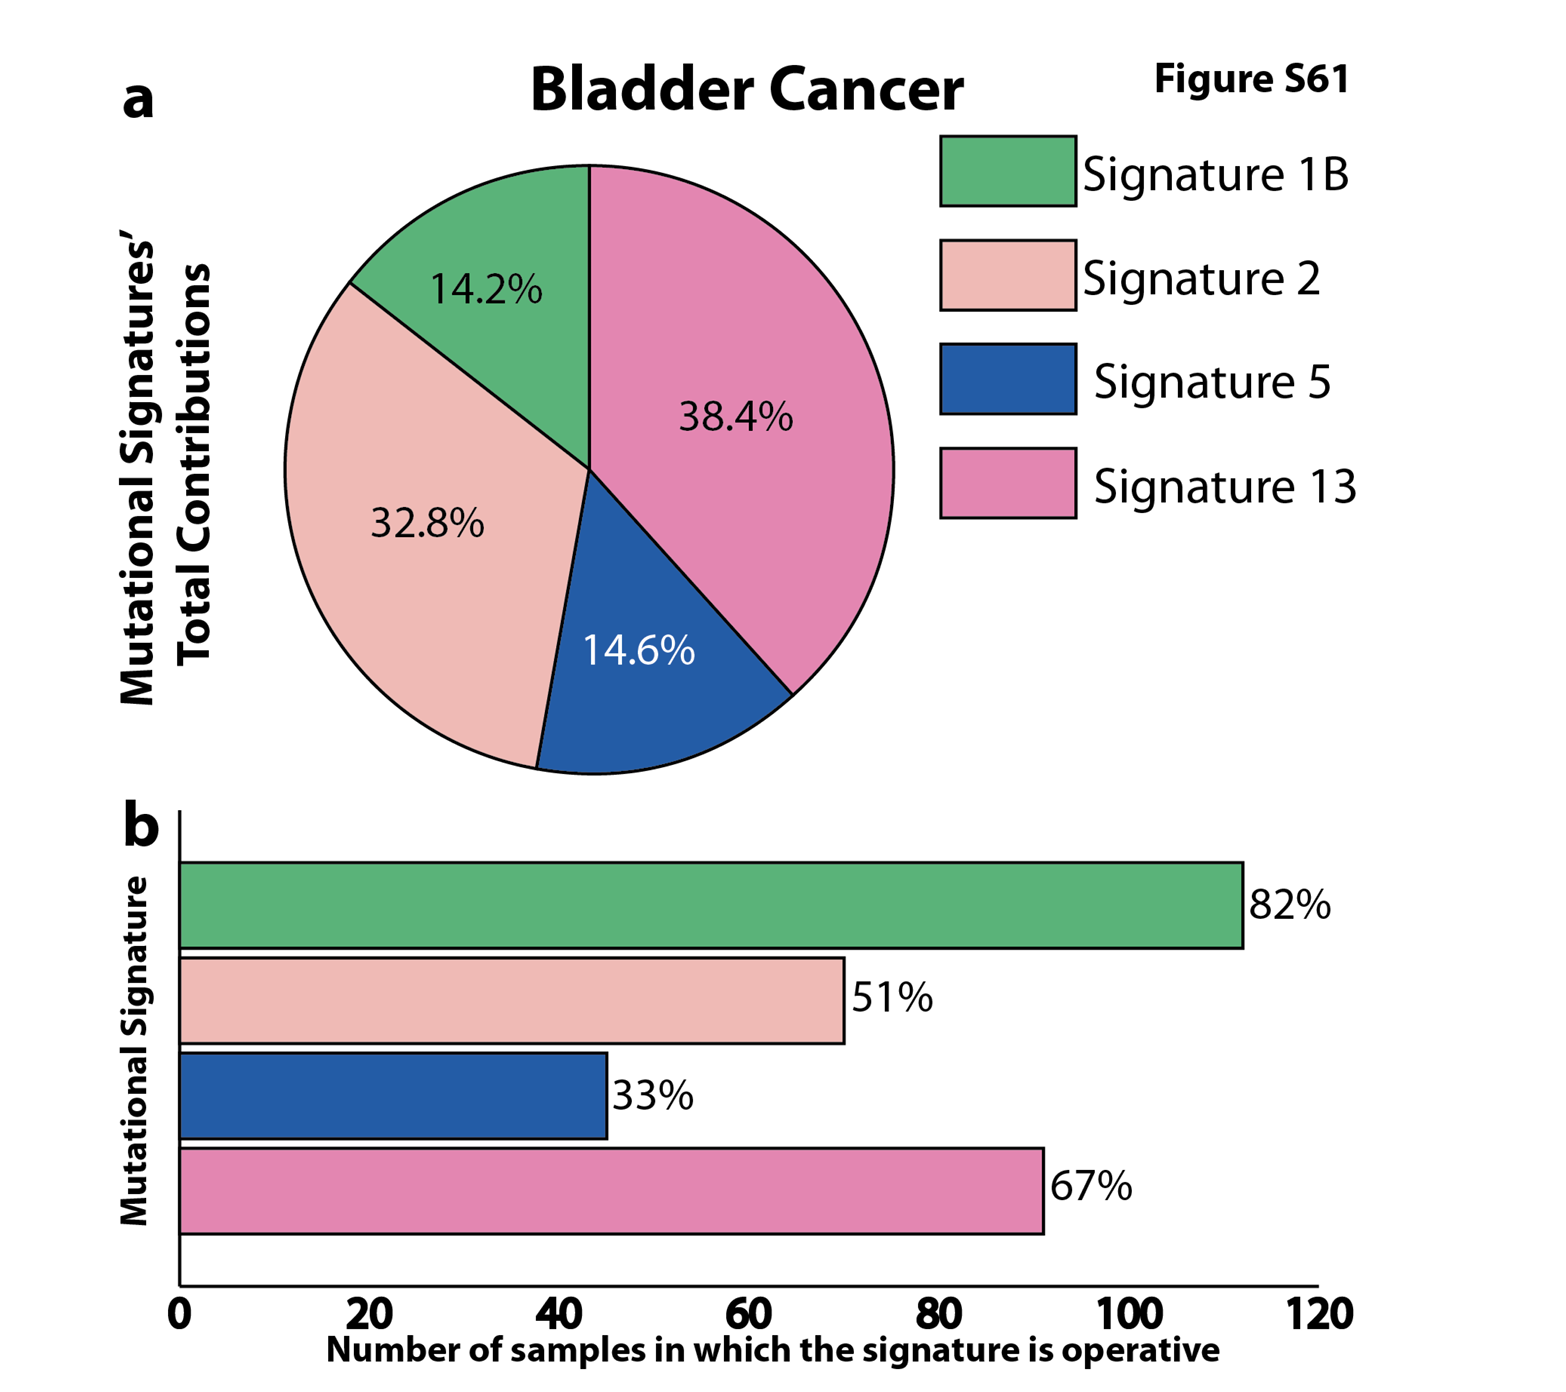
\includegraphics[width=0.6\textwidth,height=0.6\textheight,keepaspectratio]{Sections/Lit_review/Resources/bladder_mut_sig.png}
    \caption{Image from Supplementary \cite{Alexandrov2013-gi} showing the mutation signatures for bladder cancer. a) showing the the contribution of each signature while b) the number of samples where it was found. }
    \label{fig:lit:bladder_mut_sig}
\end{figure}


% epigenetic burden
The high somatic mutation burden is also highlighted by other research \cite{Tcga2014-dr, Robertson2017-mg, Kamoun2020-tj}. The first two studies found that the mutations disrupt the epigenetic machinery. Understanding these anomalies have the potential to lead to new potential targeted treatments.





\subsection{Non-cancerous dataset}

% What are the three different types of tissues used?

% From which datasets where those used? Bladder vs Uropathies

% Properties of P0, Abs-Ca and Undifferentiated. Why it is important to include all of this? Abs-Ca related more to Luminal and Undiff more to Basal

% Why are these useful?

\subsection{Conclusion}

% Talk about the

\pagebreak

\begin{todolist}
    \item Overview of the bladder cancer 
    \begin{todolist}
        \item [\done] Statistics worlwide/UK/Europe
        \item [\done] Main causes, metal contamination
        \item [\done] More prevalent in men
        \item [\done] NMIBC vs MIBC
    \end{todolist}
    \item Why it is so bad? 
    \begin{todolist}
        \item [\done] Impact of the quality of life, treatment cost?
        \item [\done] Metastasis
    \end{todolist}
    \item Efforts to solve it and introduce the subtypes problem
    \item Introduce the consensus, TCGA and Lund
    \begin{todolist}
        \item Table markers for Consensus
        \item Table markers for TCGA
        \item Table markers for Lund
        \item Mutations found and relevant
    \end{todolist}
    \item Talk about the current UK trial that is using TCGA subtypes, stressing the importance of finding the right subgroups
    \item Healthy dataset 
    \begin{todolist}
        \item different tissue types
        \item what are the sources of the dataset
        \item gene markers for each dataset
    \end{todolist}

\end{todolist}